\chapter{Context and objectives} \label{chapter2}
\minitoc
\eject

\section{Introduction}

This chapter presents the general context for this work, and leads to a definition of the problematic addressed in this thesis.
Section \ref{chapter2:web-as-a-platform} presents the context for the web development, and the motivation that led the web to become a software platform. It presents briefly the main languages available for initiating a web application, and a great section is dedicated to Javascript, as it is increasingly gained popularity these past few years.
Section \ref{chapter2:highly-concurrent-web-servers} presents the problematic for developping web server for large audiences.
It explains why the languages presented in the previous section often fail to grow with the project they initially supported very efficiently.
It conclude that this rupture is an economical risk for young projects.
Finally, section \ref{chapter2:equivalence} presents the goal of this work.
That is to reconcile the technologies used in the initial phase of a project, with the ones used to grow the project in performance.

\section{The Web as a platform}

\subsection{From operating systems to the web}


With the invention of electronic computing machine, appeared the market for software applications.
This market is not limited by marginal production cost ; software being a virtual product, the production and distribution cost for another unit is virtually null.
The market is limited by the platform a software can be deployed on.
The bigger the platform, the wider the market.
There is an economically incentive to standardize and widen the platform, both for the provider, and for the consumer.
The first platforms started as products, in competition with other products.
Their manufacturers had economical incentive to increase their market share.
Microsoft successfully took over the market of operating system in the 90s, and was on the edge of monopoly more than once.
But eventually, the product is standardized, and becomes the platform.

\begin{wrapfigure}{r}{0.2\textwidth}
  \vspace{-27pt}
  \begin{center}
    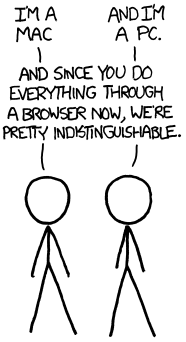
\includegraphics[width=0.18\textwidth]{../ressources/Mac-PC.png}
  \end{center}
  \vspace{-20pt}
\end{wrapfigure}

Before the internet, this market was limited for distribution by the physical medium.
It takes time to burn a CD, or a floppy, and to bring it to the consummer's home.
Sir Tim Berners Lee invented the world wide web in 1989.
It was initially intended to share scientific documents and results.
And it eventually became the distribution medium of choice for every virtual products, software included.
It pushed the scalability of software distribution.

Similarly to operating systems, Web browsers started as software products.
They exposed innovative features to try to increase their market share.
Among others is the ability to run scripts.
It allows to deploy and run software at unprecedented scales.
The web became the platform.
Now, with web services, or Software as a Service (SaaS), the distribution medium of software is so transparent that owning a software product to have an easier access is no longer relevant.
We explore now the different languages to write and deploy applications on the web.

\subsection{The languages of the web}

In the early 90's, during the web early development, most of the now popular programming languages were released.
Python(1991), Ruby(1993), Java(1994), PHP(1995) and  Javascript(1995).
With Moore's law predicting exponential increase in hardware performance, the industry realized that development time is more expensive than hardware.
Low-level languages were replaced by higher-level language, trading performance for accessibility.
The economical gain in development time compensated the worsen performances of these languages.

Java, developed by Sun Microsystems, imposes itself early as a language of choice and never really decreased.
The language is executed on a virtual machine, allowing to write an application once, and to deploy it on heterogeneous machines.
The software industry quickly adopted it as its main development language.
It is currently the second most cited language on StackOverflow, and used on Github.
And is in the first place of many language popularity indexes.
However, the software industry wants stable and safe solutions.
This prudence generally slows down Java evolution.
The language struggled to keep up with the latest trends in software development.

\textit{Python is the second best language for everything.}
It is a general purpose language, currently popular for data science.
In 2003, the release of the Django web framworks brought the language to the web development scene.

Ruby was confined in Japan and almost unknown to the world until the release of Rails in 2005.
With the release of this web framework, Ruby took-off and is still in active use.
It meets the latest trends in software development.
And it might had replaced Java if the latter had not been so well adopted in the software industry.

PHP stands for Personal Home Page Tools.
It was initially designed to build personal web pages.
It might be one of the easiest language to start web development.
However, according to several language popularity indexes, it is on a slow decline since a few years.
It is generally unfit to grow projects to industrial size.

Since a few years, Javascript is slowly becoming the main language for web development.
It is the only choice in the browser.
Because of this unavoidable position, it became fast (V8, ASM.js) and usable (ES6, ES7).
It is a target for LLVM, allowing many languages to compile to Javascript, strengthening again its omnipresent position.
Additionally, it is present on the server as well with Node.js
It is everywhere.
I argue in this thesis, that Javascript is the language of choice to bring a prototype to industrial standards.

\subsection{Explosion of Javascript popularity}

\subsubsection{In the beginning}

Javascript was created by Brendan Eich at Netscape around May 1995, and released to the public in September.
At the time, Java was quickly adopted as default language for web servers development, and everybody was betting on pushing Java to the client as well.
The history proved them wrong.

When Javascript was released in 1995, the world wide web was on the rise.\ftnt{http://www.internetlivestats.com/internet-users/}
Browsers were emerging, and started a battle to show off the best features and user experience to attract the wider public.\footnote{to get an idea of the web in 1997 : \url{http://1x-upon.com/}}
Javascript was released to be one of these features on Netscape navigator.
Microsoft released their browser Internet Explorer 3 in June 1996 with a concurrent implementation of Javascript.
At the time, because of the differences between the two implementations, web pages had to be designed for a specific browser.
This competition was fragmenting the web.

Netscape submitted Javascript to Ecma International for standardization in November 1996 to stop this fragmentation.
In June 1997, ECMA International released ECMA-262, the first specification of ECMAScript, the standard for Javascript.
A standard to which all browser should refer for their implementations.
% TODO more on the Ecma specification ?

The initial release of Javascript was designed in a rush. The version released in 1995 was finished within 10 days.
And, it was intended to be simple enough to attract unexperienced developers.
For these reasons, the language was considered poorly designed and unattractive by the developer community.

But things evolved drastically since.
The success of Javascript is due to many factors ; maybe the most important of all is the \textit{View Source} menu that reveals the complete source code of any web application.
\textit{The view source menu is the ultimate form of open source}\ftnt{http://blog.codinghorror.com/the-power-of-view-source/}.
It is the vector of the quick dissemination of source code to the community, which picks, emphasizes and reproduces the best techniques.
It brought open source and collaborative development to the web.
Moreover, all web browsers include a Javascript interpreter, making Javascript the most ubiquitous runtime in history \cite{Flanagan2006}.
% Every browser include development tools for Javascript, making it the most ubiquitous development environment, as well.

When such a language is distributed freely with the tools to reproduce and experiment on every piece of code.
And its distribution is carried during the expansion of the largest communication network in history.
Then an entire generation seizes this opportunity to incrementally build and share the best tools they can.
This collaboration is the reason for the popularity of Javascript on the Web.
% When a language is released, available freely at a world wide scale, and simple enough to be handled by a generation of teenager inspired by the technology hype, it produce an effervescent community around what is now one of the most popular and widely used programming language.

\subsubsection{Rising of the unpopular language}

\begin{figure}[h!]
{\fontfamily{phv}\fontseries{l}
\fontsize{10pt}{10pt}\selectfont
Why does Javascript suck?\ftnt{http://whydoesitsuck.com/why-does-javascript-suck/}

Is Javascript here to stay?\ftnt{http://www.javaworld.com/article/2077224/learn-java/is-javascript-here-to-stay-.html}

Why Javascript Is Doomed.\ftnt{http://simpleprogrammer.com/2013/05/06/why-javascript-is-doomed/}

Why JavaScript Makes Bad Developers.\ftnt{https://thorprojects.com/blog/Lists/Posts/Post.aspx?ID=1646}

JavaScript: The World's Most Misunderstood Programming Language\ftnt{http://www.crockford.com/javascript/javascript.html}

Why Javascript Still Sucks\ftnt{http://www.boronine.com/2012/12/14/Why-JavaScript-Still-Sucks/}

10 things we hate about JavaScript\ftnt{http://www.infoworld.com/article/2606605/javascript/146732-10-things-we-hate-about-JavaScript.html}

Why do so many people seem to hate Javascript?\ftnt{https://www.quora.com/Why-do-so-many-people-seem-to-hate-JavaScript}
}
\end{figure}

Javascript started as a programming language to implement short interactions on web pages.
The best usage example was to validate some forms on the client before sending the request to the server.
This situation hugely improved since the beginning of the language.
Nowadays, there is a lot of web-based application replacing desktop applications, like mail client, word processor, music player, graphics editor…

There is now more software services released to the public as web-based application compared to desktop clients.

ECMA International released several version in the few years following the creation of Javascript.
The first and second version, released in 1997 and 1998, brought minor revisions to the initial draft.
However, the third version, released in the late 1999, contributed to give Javascript a more complete and solid foundation as a programming language.
From this point on, the consideration for Javascript kept improving.

%An important reason for this reconsideration started in 2005.
In 2005, James Jesse Garrett released \textit{Ajax: A New Approach to Web Applications}, a white paper coining the term Ajax \cite{Garrett2005}.
This paper points the trend in using this technique, and explain the consequences on user experience.
Ajax stands for Asynchronous Javascript And XML.
It consists of using Javascript to dynamically request and refresh the content inside a web page.
It has the advantage to avoid requesting a full page from the server.
Javascript is not anymore confined to the realm of small user interactions on a terminal.
It can be proactive and responsible for a bigger part in the whole system spanning from the server to the client.
Indeed, this ability to react instantly to the user gave to developer the feature to develop richer applications inside the browser.
%, while keeping all the advantages of web-based applications.
At the time, the first web applications to use Ajax were Gmail, and Google maps\footnote{A more in-depth analysis of the history of Ajax, given by late Aaron Swartz \url{http://www.aaronsw.com/weblog/ajaxhistory}}.

Around this time, the Javascript community started to emerge.
The third version of ECMAScript had been released, and it was homogeneously supported in the browsers.
However, the DOM, and the \texttt{XMLHttpRequest} method, two components on which AJAX relies, still present heterogeneous interfaces among browsers.
Javascript framework were released with the goal to straighten the differences between browsers implementations.
Prototype\ftnt{http://prototypejs.org/} and DOJO\ftnt{https://dojotoolkit.org/} are early famous examples, and later jQuery\ftnt{https://jquery.com/} and underscore\ftnt{http://underscorejs.org/}.
These frameworks are responsible in great part to the wide success of Javascript and of the web technologies.

In the meantime, in 2004, the Web Hypertext Application Technology Working Group\ftnt{https://whatwg.org/} was formed to work on the fifth version of the HTML standard.
This new version provide new capabilities to web browsers, and a better integration with the native environment.
It features geolocation, file API, web storage, canvas drawing element, audio and video capabilities, drag and drop, browser history manipulation, and many mores.
It gave Javascript the missing interfaces to become a rich environment to develop rich application in the browser.
The first public draft of HTML 5 was released in 2008, and the fifth version of ECMAScript was released in 2009.
These two releases, ECMAScript 5 and HTML5, represent a mile-stone in the development of web-based applications.
Javascript became the programming language of this rising application platform.

Javascript, and web technologies are also used outside the web.
NW.js\ftnt{https://github.com/nwjs/nw.js} and electron\ftnt{https://github.com/atom/electron} are two solutions to deploy application built with web technologies.
They use Node.js and Chromium.
The Atom text editor\ftnt{https://atom.io/}, Popcorn Time\ftnt{https://popcorntime.io/} and Light Table\ftnt{http://lighttable.com/} are example of such applications.
However, if web applications are common choice for web service client on the desktop, HTML5 is not yet widely accepted as ready to build complete application on mobile, where performance and design are crucial.
Indeed web-technologies are often not as capable, and well integrated as native technologies.
But even for native development, Javascript seems to be a language of choice.
An example is the React Native Framework\ftnt{https://facebook.github.io/react-native/} from Facebook, which allow to use Javascript to develop native mobile applications.
They prone the philosophy \textit{"learn once, write anywhere"}, in opposition to the usual slogan \textit{"write once, run everywhere"}.\footnote{Used firstly by Sun for Java, but then stolen by many others}
% Another example is Gnome-shell. It uses Javascript to build its interface, and extensions.
% PhoneGap (Cordova) is a huge effort toward bringing web technologies to the mobile.

\nt{Insert in this section a summary table for HTML and Javascript}

\subsubsection{Current situation}

\cit{When JavaScript was first introduced, I dismissed it as being not worth my attention. Much later, I took another look at it and discovered that hidden in the browser was an excellent programming language.}{Douglas Crockford}

% \cit{JavaScript is the world's most ubiquitous computing runtime.}{John Lam}



% I want to say that Javascript took off because it was carried by the open source community.
% The goal is to introduce the following facts : JS is widely used in the open source community.
% I need to find the argument saying that open source is taking over closed sources : Javascript / open source is taking over Java / closed source.

% TO READ :
% http://www.javaworld.com/article/2077224/learn-java/is-javascript-here-to-stay-.html
% http://blog.codinghorror.com/the-power-of-view-source/
% http://blog.codinghorror.com/javascript-the-lingua-franca-of-the-web/
% http://shaver.off.net/diary/2007/05/10/the-high-cost-of-some-free-tools/


% This success is obvious on the web and in the open source communities.
The rise of Javascript is obvious on the web and particularly the open source communities.
It also seems to be rising in the software industry.
However, it is harder to give an accurate picture of the situation.
The software industry is not as clear and open as the web.
Moreover, there is no right metrics to accurately and directly measure programming language popularity.
In the following paragraphs, I report some of the best metrics and indexes available freely on the web to try to represent the situation, both in the open source community and in the more opaque software industry.
More detailed informations are available section \ref{appendix:langpop}.

\paragraph{Available resources}

The TIOBE Programming Community index is a monthly indicator of the popularity of programming languages.
Javascript ranks 6th on this index, as of April 2015, and it was the most rising language in 2014.
It uses the number of results on many search engines as a measure of the popularity of a programming language.
The results contains learning and training resources, forums logs, books and many other traces of the activity of a the community around the language.
However, the measure used by the TIOBE is controversial, and might not be representative.
It is a lagging indicator, and the number of pages doesn't represent the number of readers.

Alternatively, the PYPL index is based on Google trends to measure the number of requests on a programming language.
Javascript ranks 7th on this index, as of May 2015.
This index seems to be more accurate, as it depicts the actual interest of the community for a language.
However, it is not representative as it only takes Google search into account.

From these indexes, the major programming languages are Java, C/C++ and C\#.
The three languages are still the most widely taught, and used to write softwares.
But Javascript is rising to become an important language as well.

\paragraph{Developers collaboration platforms}

An indicator of the popularity and usage of a language is the number of developers and projects using it.

Github is the most important collaborative development platform, with around 9 millions users.
Javascript is the most used language on github since mid-2011, with more than 320 000 repositories.
The second language is Java with more than 220 000 repositories.

\nt{TODO : graph of Github repositories by languages}

StackOverflow, is the most important Q\&A platform for developers.
It is a good representation of the activity around a language.
Javascript is the second language showing the most activity on StackOverflow, with more than 840 000 questions.
The first one is Java with more than 850 000 questions.

Black Duck Software helps companies streamline, safeguard, and manage their use of open source.
For its activity, it analyzes 1 million repositories over various forges, and collaborative platforms to produce an index of the usage of programming language in open source communities.
Javascript ranks second.
C is first, and C++ third.
Along with Java, the four first languages represent about 80\% of all programming language usage.

\nt{TODO redo this graph, it is ugly.}
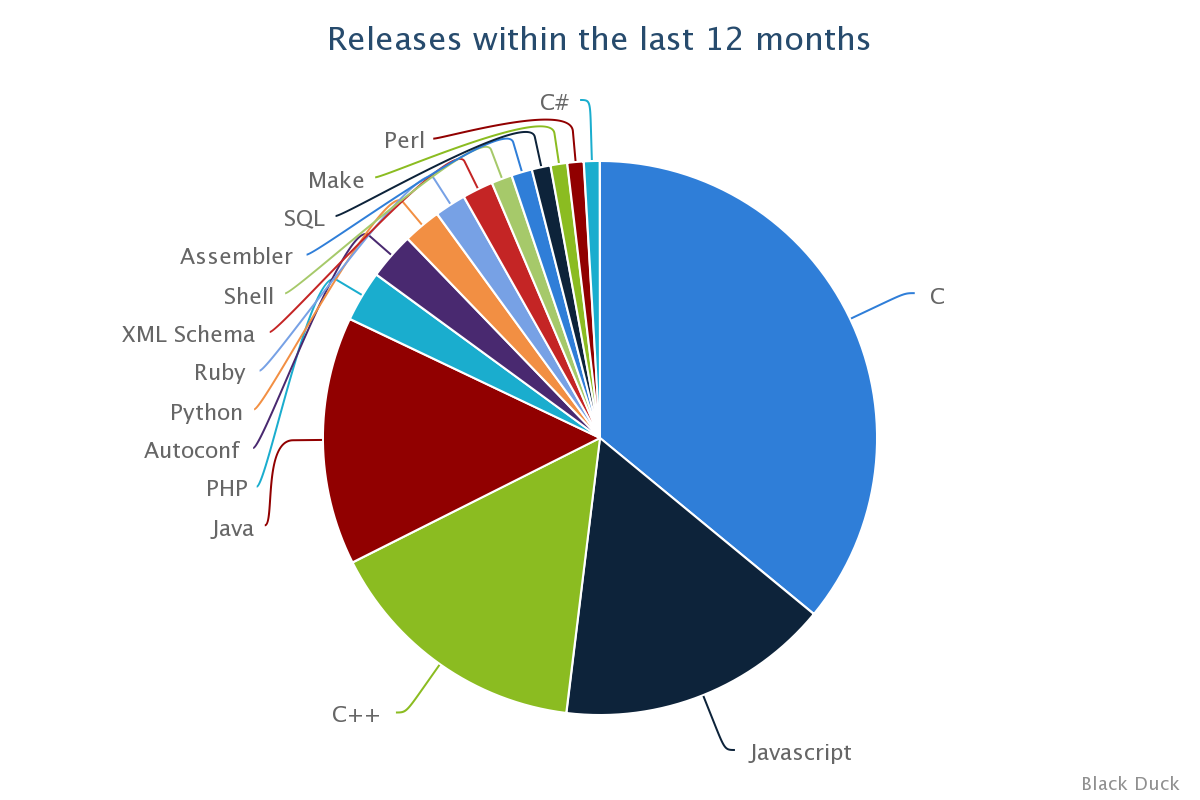
\includegraphics[width=0.9\linewidth]{../../data/js-trends/black-duck-15}

% \begin{figure}[h!]
% \begin{tikzpicture}
% [
%     pie chart,
%     slice type={c}{gray1},
%     slice type={js}{red},
%     slice type={cpp}{gray2},
%     slice type={java}{gray3},
%     slice type={php}{gray4},
%     slice type={autoconf}{gray5},
%     slice type={python}{gray6},
%     slice type={ruby}{gray1},
%     slice type={xml}{gray2},
%     slice type={sh}{gray3},
%     slice type={asm}{gray4},
%     slice type={sql}{gray5},
%     slice type={make}{gray6},
%     slice type={perl}{gray1},
%     slice type={csharp}{gray2},
%     pie values/.style={font={\small}},
%     scale=2
% ]

% \pie{}{%
%   34.80/c,%
%   15.45/js,%
%   15.13/cpp,%
%   14.02/java,%
%   2.87/php,%
%   2.65/autoconf,%
%   2.15/python,%
%   1.77/ruby,%
%   1.73/xml,%
%   1.18/sh,%
%   1.16/asm,%
%   1.07/sql,%
%   0.94/make,%
%   0.92/perl,%
%   0.90/csharp,%
% }

% \legend[shift={(1.3cm,0.9cm)}]{%
%   {C}/c,%
%   {Javascript}/js,%
%   {C++}/cpp,%
%   {Java}/java,%
%   {PHP}/php,%
%   {Autoconf}/autoconf,%
%   {Python}/python,%
%   {Ruby}/ruby,%
%   {XML Schema}/xml,%
%   {Shell}/sh,%
%   {Assembler}/asm,%
%   {SQL}/sql,%
%   {Make}/make,%
%   {Perl}/perl,%
%   {C\#}/csharp,%
% }
% \end{tikzpicture}
% \caption{Compilation results distribution}
% \end{figure}

\paragraph{Jobs}

The software industry is rather closed sourced, and its activity is rather opaque.
All these previous metrics are representing the visible activity about programming language, but are not representative of the software industry.
%To get a hint on the popularity of programming languages used in the software industry, the trends on job propositions are insightful.
The trends on job openings gives an hint of the direction the software industry is heading towards.
\textit{Indeed} provide some trends over its database of job propositions.
Javascript developers ranked at the third position, right after SQL and Java developers.
Then come C\# and C developers.
This position means that Javascript might finally be on the edge to become a major language in the software industry, and become as important as Java and C/C++.

\nt{TODO redo this graph, it is ugly.}
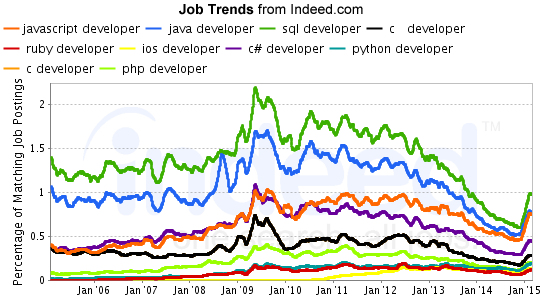
\includegraphics[width=0.9\linewidth]{../../data/js-trends/jobgraph}



All these metrics in this section represent different faces of the current situation of Javascript adoption.
With the rise of web applications, we can safely say that Javascript is one of most important language of this decade, alongside with Java and C/C++.
It is widely used in open source projects, and everywhere on the web, as well as in the software industry.
\section{Highly concurrent web servers}

\nt{This section needs review}

\subsection{Concurrency}

The Internet allows interconnection at an unprecedented scale.
There is currently more than 16 billions devices connected to the internet, and it is growing exponentially\ftnt{http://blogs.cisco.com/news/cisco-connections-counter}.
This massively interconnected network gives the ability for a web applications to be reached at the largest scale.
A large web application like google search receives about 40 000 requests per seconds.
That is about 3.5 billions requests a day\ftnt{http://www.internetlivestats.com/google-search-statistics/}.
Such a web application needs to be highly concurrent to manage a large number of simultaneous request.
Concurrency is the ability for an application to make progress on several tasks at the same time.
For example to respond to several simultaneous requests, a task is a part in the response to a request. \nt{TOOD define more clearly what is a task}
%It represents an uninterrupted flow of requests, with a growing throughput.

In the 2000s, the limit to reach was to process 10 thousands simultaneous connections with a single commodity machine\ftnt{http://www.kegel.com/c10k.html}.
Nowadays, in the 2010s, the limit is set at 10 millions simultaneous connections at roughly the same price\ftnt{http://c10m.robertgraham.com/p/manifesto.html}.
With the growing number of connected devices on the internet, concurrency is a very important property in the design of web applications.

\subsubsection{Scalability}

The traffic of a popular web application such as Google search is huge, and it remains roughly stable because of this popularity.
There is no apparent spikes in the traffic, because of the importance of the average traffic.
However, the traffic of a less popular web application is much more uncertain.
If the web application fits the market need, it might become viral when it is efficiently relayed in the media.
For example, when a web application appears in the evening news, it expects a huge spike in traffic.
With the growth of audience, the number of simultaneous requests obviously  increases, and the load of the web application on the available resources increases  as well.
The available resources needs to increase to meet the load.
This growth might be steady and predictable enough to plan the increase of resources ahead of time, or it might be erratic and challenging.
The spikes of a less popular web application are unpredictable.
Therefore, the concurrency needs to be expressed in a scalable fashion.
An application is scalable, if the growth of its audience is proportional to the increase of its load on the resources.
For example, if a scalable application uses one resource to handle $n$ simultaneous requests, it will use $k$ resource to handle two times $n$ simultaneous requests.
With $k$ being constant, for $n$ ranging from tens to millions of simultaneous requests.
Scalability assures that the resource usage is not increasing exponentially in function of the audience increase ; it increases roughly linearly.


\subsubsection{Time-slicing and parallelism}

Concurrency can be achieved on hardware with either a single or several processing units.
On a single processing unit, the tasks are executed sequentially ; their executions are interleaved in time.
On several processing unit, the tasks are executed in parallel.
Parallel executions reduce computing time over sequential execution, as it uses more processing units.

If the tasks are completely independent, they can be executed in parallel as well as sequentially.
This parallelism is a form of scalable concurrency, as it allows to stretch the computation on available hardware to meet the required performance, at the required cost.
This parallelism is used in operating system to execute several applications concurrently to allow multi-tasking.

However, the tasks of an application are rarely independent.
The tasks need to coordinate their dependencies to modify the global state of the application.
This coordination limits the possible parallelism between the tasks, and might impose to execute them sequentially.
The type of possible concurrency, sequential or parallel, is defined by the required coordination between the tasks.
Either the tasks are independents and they can be executed in parallel, or the tasks need to coordinate a common state, and they need to be executed sequentially to avoid conflicting accesses to the state.

% The same limitations are found in the two paradigms I study in this thesis : event-loop and multi-process.

\subsection{Interdependencies}

It is easier to understand the possible parallelism of a cooking recipe than an application.
That is because the modifications to the state are trivial in the cooking recipe, hence the interdependencies between operations.
It is easy to understand that preheating the oven is independent from whipping up egg whites.
While the interdependencies are not immediately obvious in an application.
\nt{TODO is this metaphor useful here ? if yes, continue to a transition}

\subsubsection{State coordination}

The interdependencies between the tasks impose the coordination of the global application state.
This coordination happen either by sending events from one task to another, or by modifying a shared memory.

If the tasks are independent enough, they never need access to a state at the same time.
The coordination of the state of the application can be done with message passing.
They pass the states from one task to another so as to always have an exclusive access on the state.
As example, applications built around a pipeline architecture define independent tasks arranged to be executed one after the other.
The tasks pass the result of their computation to the next.
These tasks never share a state.

If the tasks need concurrent accesses to a state, they cannot efficiently pass the state from one to the other repeatedly.
They need to share and to coordinate their accesses to this state.
Each access needs to be exclusive to avoid corruption.
This exclusivity is assured differently depending on the scheduling strategy.

\subsubsection{Task scheduling}

There is roughly two main scheduling strategy to execute tasks sequentially on a single processing unit : preemptive scheduling and cooperative scheduling.
The state coordination presented previously is highly depending on the scheduling strategy.

Preemptive scheduling is used in most execution environment in conjunction with multi-threading.
The scheduler allows each task to execute for a limited time before preempting it to let another task execute.
It is a fair and pessimistic scheduling, as it grant the same amount of computing time to each task.
However, as the preemption might happen at any point in the execution, it is important for the developer to lock the shared state before access, so as to assure exclusivity.
This protection is known to be hard to manage.
% This scheduling strategy should be avoided except when true concurrency is needed in concert with true shared state.
% Shared state could probably always be emulated with isolated memory and message passing.

In cooperative scheduling, the scheduler allows a task to run until the task yield the execution back.
Each task is an atomic execution ; it is never be preempted, and have an exclusive access on the memory.
It gives back to the developer the control over the preemption.
It seems to be the easiest way for developers to write concurrent programs efficiently.
Indeed, I presented in the previous section the popularity of Javascript, which is often implemented on top of this scheduling strategy (DOM, Node.js).

As I explained the different paradigms for writing concurrent program in this subsection, it appears that the main problem is to assure to the developer for each task the exclusive access to the state of its application.
This assurance is called invariance.

\subsubsection{Invariance}

I call invariance the assurance given that the state accessible from a task will remain unchanged during its access to avoid corruption, and more generally to allow the developer to perform atomic modifications on the state.
This assurance allows the developer to regroup operations logically so as to perform all the operations without interference from concurrent executions.
The same concept is found in transactional memory.

In a multi-process application, there is no risk of corrupted state by simultaneous, conflicting accesses.
The invariance is made explicit by the developer as the memory needs to be isolated inside each process.
The invariance is assure at any point in time because the process remain isolated.

In a cooperative scheduling application, the developer is aware of the points in the code where the scheduler switches from one concurrent execution to the other, so it can manage its state in atomic modification.
The invariance is assured, because any region in the memory can be accessed only by one task at a time.

Between these two invariances, the locking mechanisms seems to be a promising compromise.
The developer defines only the shared states, and these are locked only when needed.
However, it increases the complexity of the possible locked combination, leading to unpredictable situations, such as deadlock, and so on.
The locking mechanisms are known to be difficult to manage, and sub-optimal.
Indeed, they are eventually as efficient as a queue to share resources.

For the rest of this thesis, I focus only on the invariances provided by the multi-process paradigm and the cooperative scheduling.
They are similar, because the developer defines sequence of instructions with atomic access to the memory.
And in both paradigms, these sequences communicate by sending messages to each other.
The difference is that in the multi-process paradigm, the developer defines the region and the isolated memory, while in the cooperative scheduling, the developer defines only the region, and the memory is isolated by the exclusivity in the execution.

This difference seems to be crucial in the adoption of the technology by the developer community.
As we will see in the next subsection, the parallelism of multi-process is difficult to develop, but provide good performances, while the sequentiality of the cooperative scheduling is easier to develop, but provide poor performances compared to parallelism.


\nt{TODO this paragraph needs review}

\subsection{Technological shift}

% \subsubsection{Power wall}

\subsubsection{Scalable concurrency}

Around 2004, the so-called Power Wall was reached.
The clock of CPU is stuck at 3GHz because of the inability to dissipate the heat generated at higher frequencies.
Additionally, the instruction-level parallelism is limited.
Because of these limitations, a processor is limited in the number of instruction per second it can execute.
Therefore, a coarser level of parallelism, like the task-level, multi-processes parallelism previously presented is the only option to achieve high concurrency and scalability.
But as I presented previously, this parallelism requires the isolation of the memory of each independent task.
This isolation is in contradiction with the best practices of software development, hence, is difficult to develop for common developers.
It creates a rupture between performance and development accessibility.

\subsubsection{The case for global memory}

The best practices in software development advocate to design a software into isolated modules.
This modularity allows to understand each module by itself, without an understanding of the whole application.
The understanding of the whole application emerges from the interconnections between the different modules.
A developer need only to understand a few modules to contribute to an application of hundreds or thousands of modules.

Modularity advocates three principles : encapsulation, a module contains the data, as well as the functions to manipulate this data ; separation of concerns, each module should have a clear scope of action, and this scope should not overlap with the scope of other modules ; and loose coupling, each module should require no, or as little knowledge as possible about the definition of other modules.
The main goal followed by these principles, is to help the developer to develop and maintain a large code-base.

Modularity is intended to avoid a different problem than the isolation required by parallelism.
The former intends to avoid unintelligible spaghetti code ; while the latter avoids conflicting memory accesses resulting in corrupted state.
The two goals are overlapping in the design of the application.
\nt{TODO needs more explanations -> so it is hard for dev to do both ? Why exactly ?}
Therefore, every language needs to provide a compromise between these two goals, and specialized in specific type of applications.
I argue that the more accessible, hence popular programming languages choose to provide modularity over isolation.
They provide a global memory at the sacrifice of the performance provided by parallelism.
On the other hand, the more efficient languages sacrifice the readability and maintainability, to provide a model closer to parallelism, to allow better performances.
\nt{TODO instead of language, use a more generic term to refer to language or infrastructure}
\nt{TODO justification and examples. What are modular application, or parallel applications ?}


\subsubsection{Rupture}

Between the early development, and the maturation of a web application, the development needs are radically different.
In its early development, a web application needs to quickly iterate over feedback from its users.
\textit{``Release early, release often''}, and \textit{``Fail fast''} are the punchlines of the web entrepreneurial community.
The development team quickly releases a Minimum Viable Product as to get these feedbacks.
The development reactivity is crucial.
The first reason of startup failures is the lack of market need\ftnt{https://www.cbinsights.com/blog/startup-failure-post-mortem/}.
Therefore, the development team opt for a popular, and accessible language.

As the application matures and its audience grows, the focus shift from the development speed to the scalability of the application.
% The ability of the application to handle a large amount of simultaneous request.
The development team shift from a modular language, to a language providing parallelism.


This shift brings two problems.
First, the development team needs to take a risk to be able to grow the application.
This risk usually implies for the development team to rewrite the code base to adapt it to a completely different paradigm, with imposed interfaces.
It is hard for the development team to find the time, hence the money, or the competences to deploy this new paradigm.
Indeed, the number two and three reasons for startup failures are running out of cash, and missing the right competences.
Second, after this shift the development pace is different.
Parallel languages are incompatible with the commonly learned design principles.
The development team cannot react as quickly to user feedbacks as with the first paradigm.

% There is a performance problem with languages about concurrency.
% The used imperative programming languages are difficulty parallel.
% And the highly parallel programming languages are not largely used.

% There is a technological rupture between the two.

This technological rupture proves that there is economically a need for a a more sustainable solution to follow the evolution of a web application.
A paradigm that it is easy to develop with, as needed in the beginning of a web application development, and yet scalable, so as to be highly concurrent when the application matures.

% Such a paradigm would allow to develop with a global memory, so as to follow the best practices of software development, and be able to isolate the state of each concurrent tasks to parallelize them.

\endinput










\section{From Continuations to Dues} \label{chapter5:equivalence}

This section presents the transformation from a nested imbrication of continuations into a chain of Dues.
It explains the three limitations imposed by the compiler for this transformation to preserve the semantic.
They preserve the execution order, the execution linearity and the scopes of the variables used in the operations.

\subsection{Execution order}

The compiler spots function calls with a continuation, which are similar to the abstraction in (\ref{eq:order:source}).
It wraps the function $fn$ into the function $fn_\textbf{due}$ to return a Due.
And it relocates the continuation in a call to the method $\textbf{then}$, which references the Due previously returned.
The result should be similar to (\ref{eq:order:target}).
The differences are highlighted in bold font.
\begin{equation} \label{eq:order:source}
fn([arguments], continuation)
\end{equation}
\begin{equation} \label{eq:order:target}
fn_\textbf{due}([arguments])\textbf{.then}(continuation)
\end{equation}

The execution order is different whether $continuation$ is called synchronously, or asynchronously.
If $fn$ is synchronous, it calls the $continuation$ within its execution.
It might execute $statements$ after executing $continuation$, before returning.
If $fn$ is asynchronous, the continuation is called after the end of the current execution, after $fn$.
The transformation erases this difference in the execution order.
In both cases, the transformation relocates the execution of $continuation$ after the execution of $fn$.
For synchronous $fn$, the execution order changes ; the execution of $statements$ at the end of $fn$ and the continuation switch.
The latter must be asynchronous to preserve the execution order.

\subsection{Execution linearity}

The compiler transforms a nested imbrication of continuations, which is similar to the abstraction in (\ref{eq:state:source}) into a flatten chain of calls encapsulating them, like in (\ref{eq:state:target}).
\begin{align} \label{eq:state:source}
&fn1([arguments], cont1 \{\nonumber\\
&\qquad  declare ~ variable \leftarrow result\nonumber\\
&\qquad  fn2([arguments], cont2 \{\nonumber\\
&\qquad\qquad    print ~ variable\nonumber\\
&\qquad  \})\nonumber\\
&\})
\end{align}
\begin{align} \label{eq:state:target}
&\textbf{declare variable}\nonumber\\
&fn1_\textbf{due}([arguments])\nonumber\\
&\textbf{.then}(cont1\{\nonumber\\
&\qquad  variable \leftarrow result\nonumber\\
&\qquad  fn2_\textbf{due}([arguments])\nonumber\\
&\})\nonumber\\
&\textbf{.then}(cont2\{\nonumber\\
&\qquad  print ~ variable\nonumber\\
&\})
\end{align}

An imbrication of continuations must not contain any loop, nor function definition that is not a continuation.
Both modify the linearity of the execution flow which is required for the equivalence to keep the semantic.
A call nested inside a loop returns multiple Dues, while only one is returned to continue the chain.
A function definition breaks the execution linearity.
It prevents the nested call to return the Due expected to continue the chain.
% And a call nested inside a function definition is unable to return the Due to continue the chain.
On the other hand, conditional branching leaves the execution linearity and the semantic intact.
If the nested asynchronous function is not called, the execution of the chain stops as expected.

% We demonstrate the equivalence with a sequence of two continuations.
% The equivalence is sound for a sequence of \textit{n} continuations.

\subsection{Variable scope}

In (\ref{eq:state:source}), the definitions of $cont1$ and $cont2$ are
overlapping. The $variable$ declared in $cont1$ is accessible in $cont2$ to be
printed. In (\ref{eq:state:target}), however, definitions of $cont1$ and
$cont2$ are not overlapping, they are siblings. The $variable$ is not
accessible to $cont2$. It must be relocated in a parent function to be
accessible by both $cont1$ and $cont2$. To detect such variables, the compiler
must infer their scope statically. Languages with a lexical scope define the
scope of a variable statically. Most imperative languages present a lexical
scope, like C/C++, Python, Ruby or Java. The subset of Javascript excluding
the built-in functions \texttt{with} and \texttt{eval} is also lexically
scoped. To compile Javascript, the compiler must exclude programs using these
two statements.
